\raggedbottom
\chapter{Databáze}
\label{chap:databaze}

V této práci jsme využívali dvě databáze fotopletysmografických signálů: \textit{CapnoBase} a \textit{\acl{BUT PPG}}, pro kterou budeme v této práci používat zkrácený název \acs{BUT PPG}.

Na těchto databázích jsme testovali a porovnávali výsledky použitých algoritmů.
U databáze CapnoBase jsme porovnávali naměřené systolické vrcholy s referenčními hodnotami a díky tomu jsme porovnávali i rozdíl v srdeční tepové frekvenci (\acs{TF}).
U databáze \acs{BUT PPG} nebyly referenční hodnoty systolických vrcholů k dispozici, ale byly zde referenční hodnoty \acs{TF} signálů, které jsme porovnávali s naměřenými výsledky.

\section{CapnoBase}
\label{sec:capnobase}
% Představit databázi CapnoBase, její vlastnosti a použití
CapnoBase je veřejně dostupná databáze, která obsahuje osmiminutové záznamy od 42 dětských i dospělých pacientů, podstupujících plánované chirurgické zákroky včetně anestézie~\cite{CapnoBase}.

Součástí databáze jsou \acs{PPG}, \acs{EKG} a respirační signály, se vzorkovací frekvencí 300~Hz.
Pro každý záznam jsou navíc ručně označeny systolické vrcholy v \acs{PPG}, odvozené z \acs{EKG}, což umožňuje přesné ověření správnosti detekce tepů.
Autoři však nedoporučují databázi používat k trénování či dolaďování algoritmů~\cite{CapnoBase}.
Proto jsme ji použili pouze k testování použitých algoritmů a k porovnání výsledků s referenčními hodnotami.

Díky svým vlastnostem je CapnoBase vhodná k~posouzení robustnosti a přesnosti metod v~klinických situacích~\cite{Karlen2013,Charlton2022}.

\section{\acs{BUT PPG}}
\label{sec:but_ppg}
% Databáze \acs{BUT PPG} obsahuje 3888 signálů odvozených z původních 48 záznamů, z nichž jsme úspěšně zpracovali 3672.
% Zbylých 216 úseků bylo vyloučeno kvůli chybovým stavům referenčního algoritmu.
% toto by mělo být v kapitole o databázi s odkazem na přílohu
Databáze \acs{BUT PPG} vznikla na Fakultě elektrotechniky a komunikačních technologií \acs{VUT} za účelem zkoumání kvality \acs{PPG} záznamů a odhadu \acs{TF}.
V nové rozšířené verzi obsahuje 3,888 desetisekundových měření od 50 dobrovolníků (25 žen a 25 mužů) ve věku 19 až 76~let, a to v klidu i při různých typech pohybových aktivit.
Fotopletysmografické záznamy byly pořízeny chytrými telefony \textit{Xiaomi~Mi9} a \textit{Huawei~P20~Pro} se vzorkovací frekvencí 30~Hz.
Pro referenční \acs{EKG} a akcelerometrická (\acs{ACC}) data byl použit mobilní senzor \textit{Bittium Faros~360 (nebo 180)} se vzorkovacími frekvencemi 1,000~Hz pro \acs{EKG} a 100~Hz pro \acs{ACC}~\cite{BUT_PPG,BUT_PPG_database}.
Surový \acs{PPG} signál byl extrahován z červené složky nahraného videa (viz. Obr.~\ref{fig:videoZaznamPPG}).

Každý \acs{PPG} záznam byl synchronizován s \acs{EKG} a rozdělen do desetisekundových segmentů, které následně hodnotilo tři až pět expertů~\cite{BUT_PPG_database}.
Pro označení kvality vycházeli výhradně z rozdílu mezi \acs{TF} odhadnutou z \acs{PPG} a referenční tepovou frekvencí z \acs{EKG}.
Pokud byla odchylka do pěti úderů za minutu, bylo dané měření označeno jako \uv{dobré} (1), jinak jako \uv{špatné} (0).
Tato hranice vychází z mezinárodní normy IEC~60601-2-27 a v databázi \acs{BUT PPG} je aplikována ještě přísněji~\cite{BUT_PPG}.

Přibližně polovina záznamů vznikla přiložením prstu na zadní kameru a \acs{LED}, druhá pak snímáním ucha v poloze připomínající telefonování.
V novější části databáze se rozšiřuje množství subjektů i situací, včetně manipulací s osvětlením, vyšším tlakem prstu na čočku, mluvením či chůzí, a nově se přidávají i údaje o krevním tlaku, glykémii a saturaci krve kyslíkem.

Díky této variabilitě podmínek a bohatým anotacím je \acs{BUT PPG} unikátním zdrojem pro testování robustnosti algoritmů detekce \acs{TF} a pro posuzování použitelnosti krátkých \acs{PPG} signálů z mobilního telefonu v reálné praxi.

\begin{figure}[ht]
	\centering
	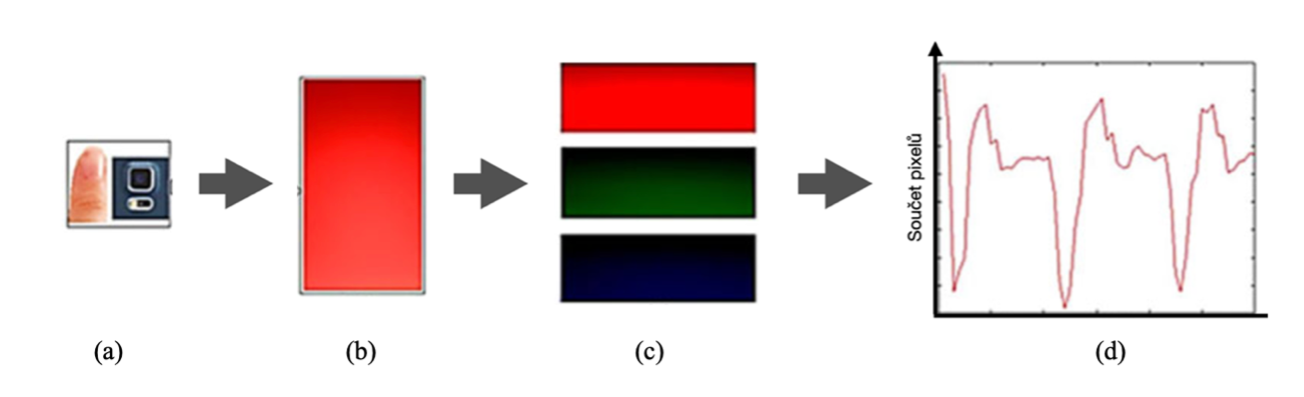
\includegraphics[width=0.8\textwidth]{./obrazky/videoZaznamPPG.png}
	\caption[Získání PPG signálu pro databázi \acs{BUT PPG}]{Záznam videa na kameru mobilního telefonu (a), jeden vybraný snímek ze záznamu (b), snímek rozložen na tři barevné složky (c), PPG signál vykreslený z červené složky (d), upraveno z~\cite{Siddiqui2016}.}
	\label{fig:videoZaznamPPG}
\end{figure}

Spojením klinicky orientované databáze CapnoBase a mobilně zaměřené \acs{BUT PPG} vzniká možnost vzájemného porovnání a ověření přesnosti algoritmů, které musejí obstát v rozdílných kontextech: v relativně stabilním klinickém prostředí a v krátkých záznamech z chytrého telefonu.